\clearemptydoublepage
\chapter{Contexte -- Cloud, ordonnancement et élasticité}
\label{chapter:context}

Dans ce deuxième chapitre, nous donnons une définition formelle du cloud, au travers des propriétés spécifiques à ces environnements de calcul et de stockage partagés. Nous présentons également quelques techniques et technologies socles dans les centres de données. Enfin, nous commentons les caractéristiques des applications déployées dans le cloud, et terminons par introduire le modèle serverless pour le cloud, qui constitue l'environnement au cœur des problématiques traitées au cours de cette thèse.

\section{\textit{Cloud computing} : une définition}

Les premières réflexions autour de l'émergence d'un système informatique à temps partagé remontent au début des années 1960~\cite{greenberger1962management}. L'idée, nouvelle, est alors de permettre le partage des ressources matérielles d'une part entre différentes tâches, et d'autre part entre différents utilisateurs~\cite{meyerVirtualMachineTimesharing1970}. L'objectif est de maximiser l'utilisation des ressources en permettant à plusieurs utilisateurs d'exploiter la même machine simultanément, limitant ainsi le gaspillage de temps de calcul~\cite{corbato1962experimental}.

Le cloud est vu comme la suite logique au succès de ces systèmes à temps partagé~\cite{hayesCloudComputing2008}. Salesforce fait partie des premières sociétés à avoir fait le pari du cloud en 1999~\cite{weissmanDesignForceCom2009} en proposant à ses clients une suite logicielle d'informatique de gestion accessible en ligne. En 2006, Amazon Web Services (\gls{AWS}) propose EC2~\footnote{\href{https://aws.amazon.com/fr/ec2/}{https://aws.amazon.com/fr/ec2/}} (pour \textit{Elastic Compute Cloud}), la première offre d'infrastructure en tant que service. La même année, Google lance Google Docs~\footnote{\href{https://www.google.fr/intl/fr/docs/about/}{https://www.google.fr/intl/fr/docs/about/}}, une suite bureautique accessible en ligne et destinée aux utilisateurs finaux. En 2010, la NASA annonce la publication sous licence libre d'OpenStack~\footnote{\href{https://www.openstack.org/}{https://www.openstack.org/}}, une plateforme logicielle permettant de gérer une infrastructure cloud, ouvrant la possibilité à de nouveaux acteurs de rentrer sur le marché du cloud sans avoir à développer une pile logicielle complète.

Le cloud apparaît donc comme un environnement hautement hétérogène pour lequel il convient d'avoir des éléments de définition communément admis.

\subsection{Caractéristiques}

Le \gls{NIST} donne une définition formelle du cloud~\cite{mellNISTDefinitionCloud} en établissant les caractéristiques essentielles d'une telle plateforme :

\begin{itemize}
    \item \textbf{Service à la demande} -- Les clients réservent des ressources matérielles de manière autonome, par exemple au travers d'une interface web, sans interagir avec un opérateur. En retour, ils n'ont généralement pas de contrôle fin sur la localité précise des ressources réservées ;
    \item \textbf{Accessible par le réseau} -- Ces ressources sont immédiatement mises à disposition des clients et accessibles par Internet ;
    \item \textbf{Partage des ressources} -- La puissance de calcul, les capacités de stockage et la bande passante sont partagées entre les clients du fournisseur de services. Des techniques de virtualisation sont mises en œuvre pour isoler les tâches déployées ;
    \item \textbf{Élasticité rapide} -- Les clients peuvent à tout moment décider d'augmenter ou de diminuer la quantité et les caractéristiques des ressources qu'ils réservent, de manière à garantir les performances de leurs applications ou maîtriser leurs coûts ;
    \item \textbf{Service mesuré} -- Les infrastructures cloud sont instrumentées de manière à fournir aux clients une information précise sur leur consommation de ressources, et les coûts monétaires associés.
\end{itemize}

\subsection{Modèles de service}

\begin{figure}[!ht]
    \centering
	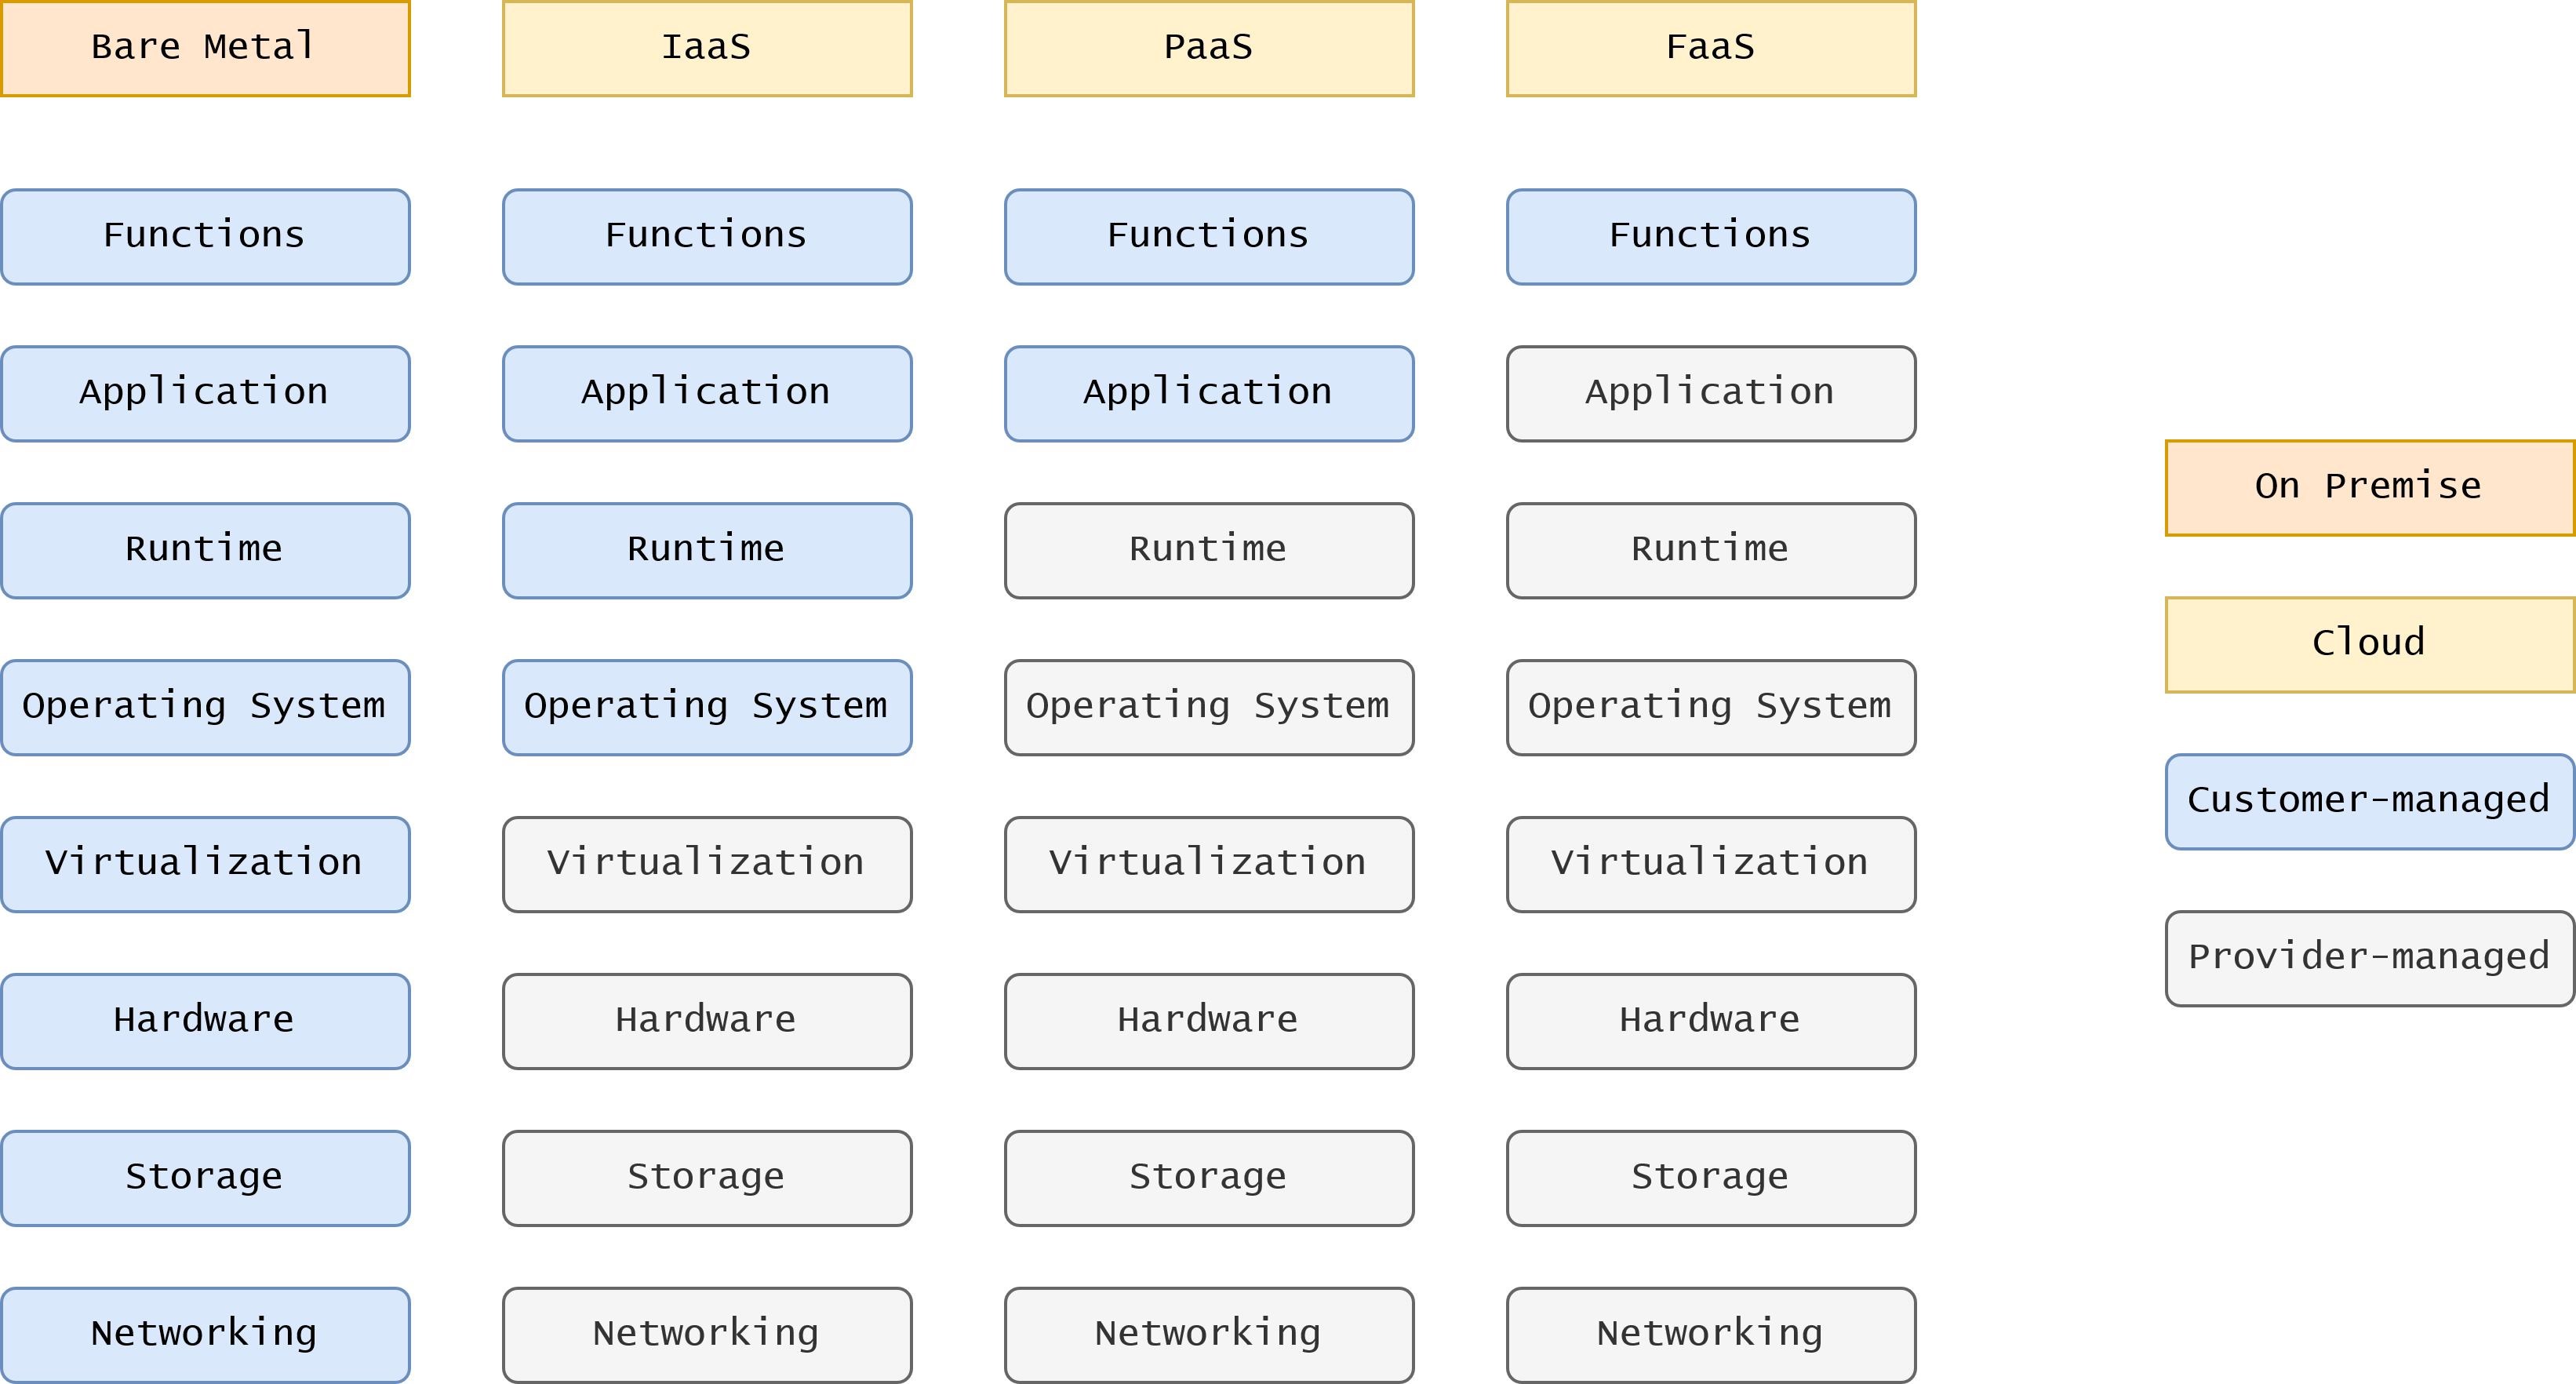
\includegraphics[width=\textwidth]{2_Chapitre2/figures/service-models.png}
	\caption[Comparaison entre différents modèles de service pour le cloud en termes de responsabilités pour le client et le fournisseur de service.]{Comparaison entre différents modèles de service pour le cloud en termes de responsabilités pour le client et le fournisseur de service (inspiré de la documentation Red Hat~{\protect \footnotemark}).}
	\label{figure:context-service-model}
\end{figure}

\footnotetext{\href{https://www.redhat.com/en/topics/cloud-computing/iaas-vs-paas-vs-saas}{https://www.redhat.com/en/topics/cloud-computing/iaas-vs-paas-vs-saas}}

Ces caractéristiques sont déclinées dans trois modèles de service, comme illustré par la figure~\ref{figure:context-service-model}, qui constituent des déclinaisons de l'offre commerciale des fournisseurs de service cloud :

\begin{itemize}
    \item \textbf{Infrastructure as a Service} (\gls{IaaS}) -- Cible les clients qui souhaitent un contrôle à grain fin sur leurs infrastructures. Les clients sont responsables de l'administration des ressources matérielles mises à leur disposition, c'est-à-dire des serveurs, souvent virtuels (voir section~\ref{section:background-virtualization}) ;
    \item \textbf{Platform as a Service} (\gls{PaaS}) -- Cible les clients qui souhaitent déployer leurs applications sans avoir la responsabilité d'administration des serveurs ;
    \item \textbf{Software as a Service} (\gls{SaaS}) -- Cible l'utilisateur final en offrant l'accès à une application entièrement administrée par le fournisseur de services.
\end{itemize}

\subsection{Modèles de déploiement}

Pour organiser les calculs et les données dans le cloud, il existe plusieurs stratégies qui correspondent à différentes contraintes métier pour les utilisateurs :

\begin{itemize}
    \item \textbf{Cloud privé} -- L'infrastructure est dédiée à une organisation qui regroupe plusieurs utilisateurs finaux. Ce modèle de déploiement est privilégié par les clients pour la sécurité et la confidentialité des données ;
    \item \textbf{Cloud public} -- L'infrastructure est partagée entre de nombreux clients hétérogènes, professionnels comme particuliers. Ce modèle de déploiement est souvent moins coûteux pour le client qu'une offre de cloud privé ;
    \item \textbf{Cloud communautaire} -- L'infrastructure est partagée entre différents acteurs ayant souvent des problématiques métier similaires (secteurs bancaire ou hospitalier par exemple) ;
    \item \textbf{Cloud hybride} -- Solution de répartition des tâches entre cloud privé et cloud public, en fonction de leur niveau de criticité.
\end{itemize}

\section{Ordonnancement dans le cloud}

Dans cette section, nous présentons les techniques mises en œuvre par les fournisseurs de services cloud pour partager les ressources matérielles et isoler les charges de travail de leurs différents utilisateurs. Nous introduisons les défis pour la mise à l'échelle de ces ressources lors de variations de charge sur les applications déployées, notamment en matière de qualité de service.

\subsection{Virtualisation dans un cadre multi-tenant}
\label{section:background-virtualization}

Le modèle économique des fournisseurs de services pour le cloud repose sur la mutualisation des ressources matérielles entre de nombreux clients~\cite{hayesCloudComputing2008}. Les plateformes cloud doivent donc prendre en charge un nombre important de traitements, ce qui entraîne une situation de partage massif des ressources matérielles qui nécessite des techniques d'isolation et de virtualisation adéquates~\cite{vaqueroLockingSkySurvey2011}. C'est ce que l'on appelle le cadre multi-tenant~\cite{weissmanDesignForceCom2009}.

Comme les ressources sont mises en commun et que différentes applications les utilisent, cela ouvre des canaux, auxiliaires ou non, vecteurs potentiels d'attaques entre les processus dans l'espace utilisateur~\cite{pedersen2017trash, wu2018side}. Bénéficier du cadre multi-tenant s'accompagne donc de la responsabilité, pour le fournisseur, de garantir la confidentialité et la sécurité des données et des différentes charges de travail des clients~\cite{vaqueroLockingSkySurvey2011}.

Pour respecter ces garanties, les fournisseurs doivent recourir à des mesures de protection pour assurer le cloisonnement entre différents processus appartenant à des applications et/ou des utilisateurs différents. Ce mécanisme consistant à présenter, de manière transparente, un environnement d'exécution distinct avec un espace d'adressage, un système de fichiers et des autorisations propres à chaque processus est appelé isolation~\cite{fehlingCloudComputingPatterns2014}. À cette fin, les fournisseurs peuvent s'appuyer sur des technologies de virtualisation.

La virtualisation est une technique d'isolation qui permet d'exécuter une application dans les limites d'un environnement d'exécution sécurisé, en introduisant une couche d'indirection entre la plateforme hôte et l'application elle-même~\cite{singhviAtollScalableLowLatency2021}.

La virtualisation des ressources de l'hôte peut se faire à l'aide de machines virtuelles (\gls{VM}, pour \textit{Virtual Machine}) ou de conteneurs. Ces environnements d'exécution donnent aux processus sous-jacents l'illusion d'avoir une machine entière à leur disposition. Alors que les \gls{VM} virtualisent les ressources physiques de l'hôte, en s'appuyant sur l'architecture du processeur pour réaliser l'isolation, les conteneurs exploitent des directives du système d'exploitation hôte pour isoler les charges de travail~\cite{mancoMyVMLighter2017}.

Lorsqu'ils choisissent le modèle d'isolation sur lequel ils souhaitent s'appuyer pour exploiter le partage des ressources, les fournisseurs cloud doivent faire un compromis entre performances et sécurité. Les conteneurs sont fréquemment la cible d'attaques par élévation de privilèges~\cite{zomer2022containers, redhat2019containers}, mais leurs temps de démarrage sont de plusieurs ordres de grandeur inférieurs à ceux des machines virtuelles : le temps d'initialisation des conteneurs se compte en centaines de millisecondes, tandis que les \gls{VM} démarrent en quelques secondes~\cite{mancoMyVMLighter2017}. La conception de machines virtuelles légères offrant des temps d'initialisation comparables à ceux des conteneurs est un sujet de recherche essentiel~\cite{agacheFirecrackerLightweightVirtualization, Anjali2020BlendingCA}.

\begin{figure}[!ht]
    \centering
	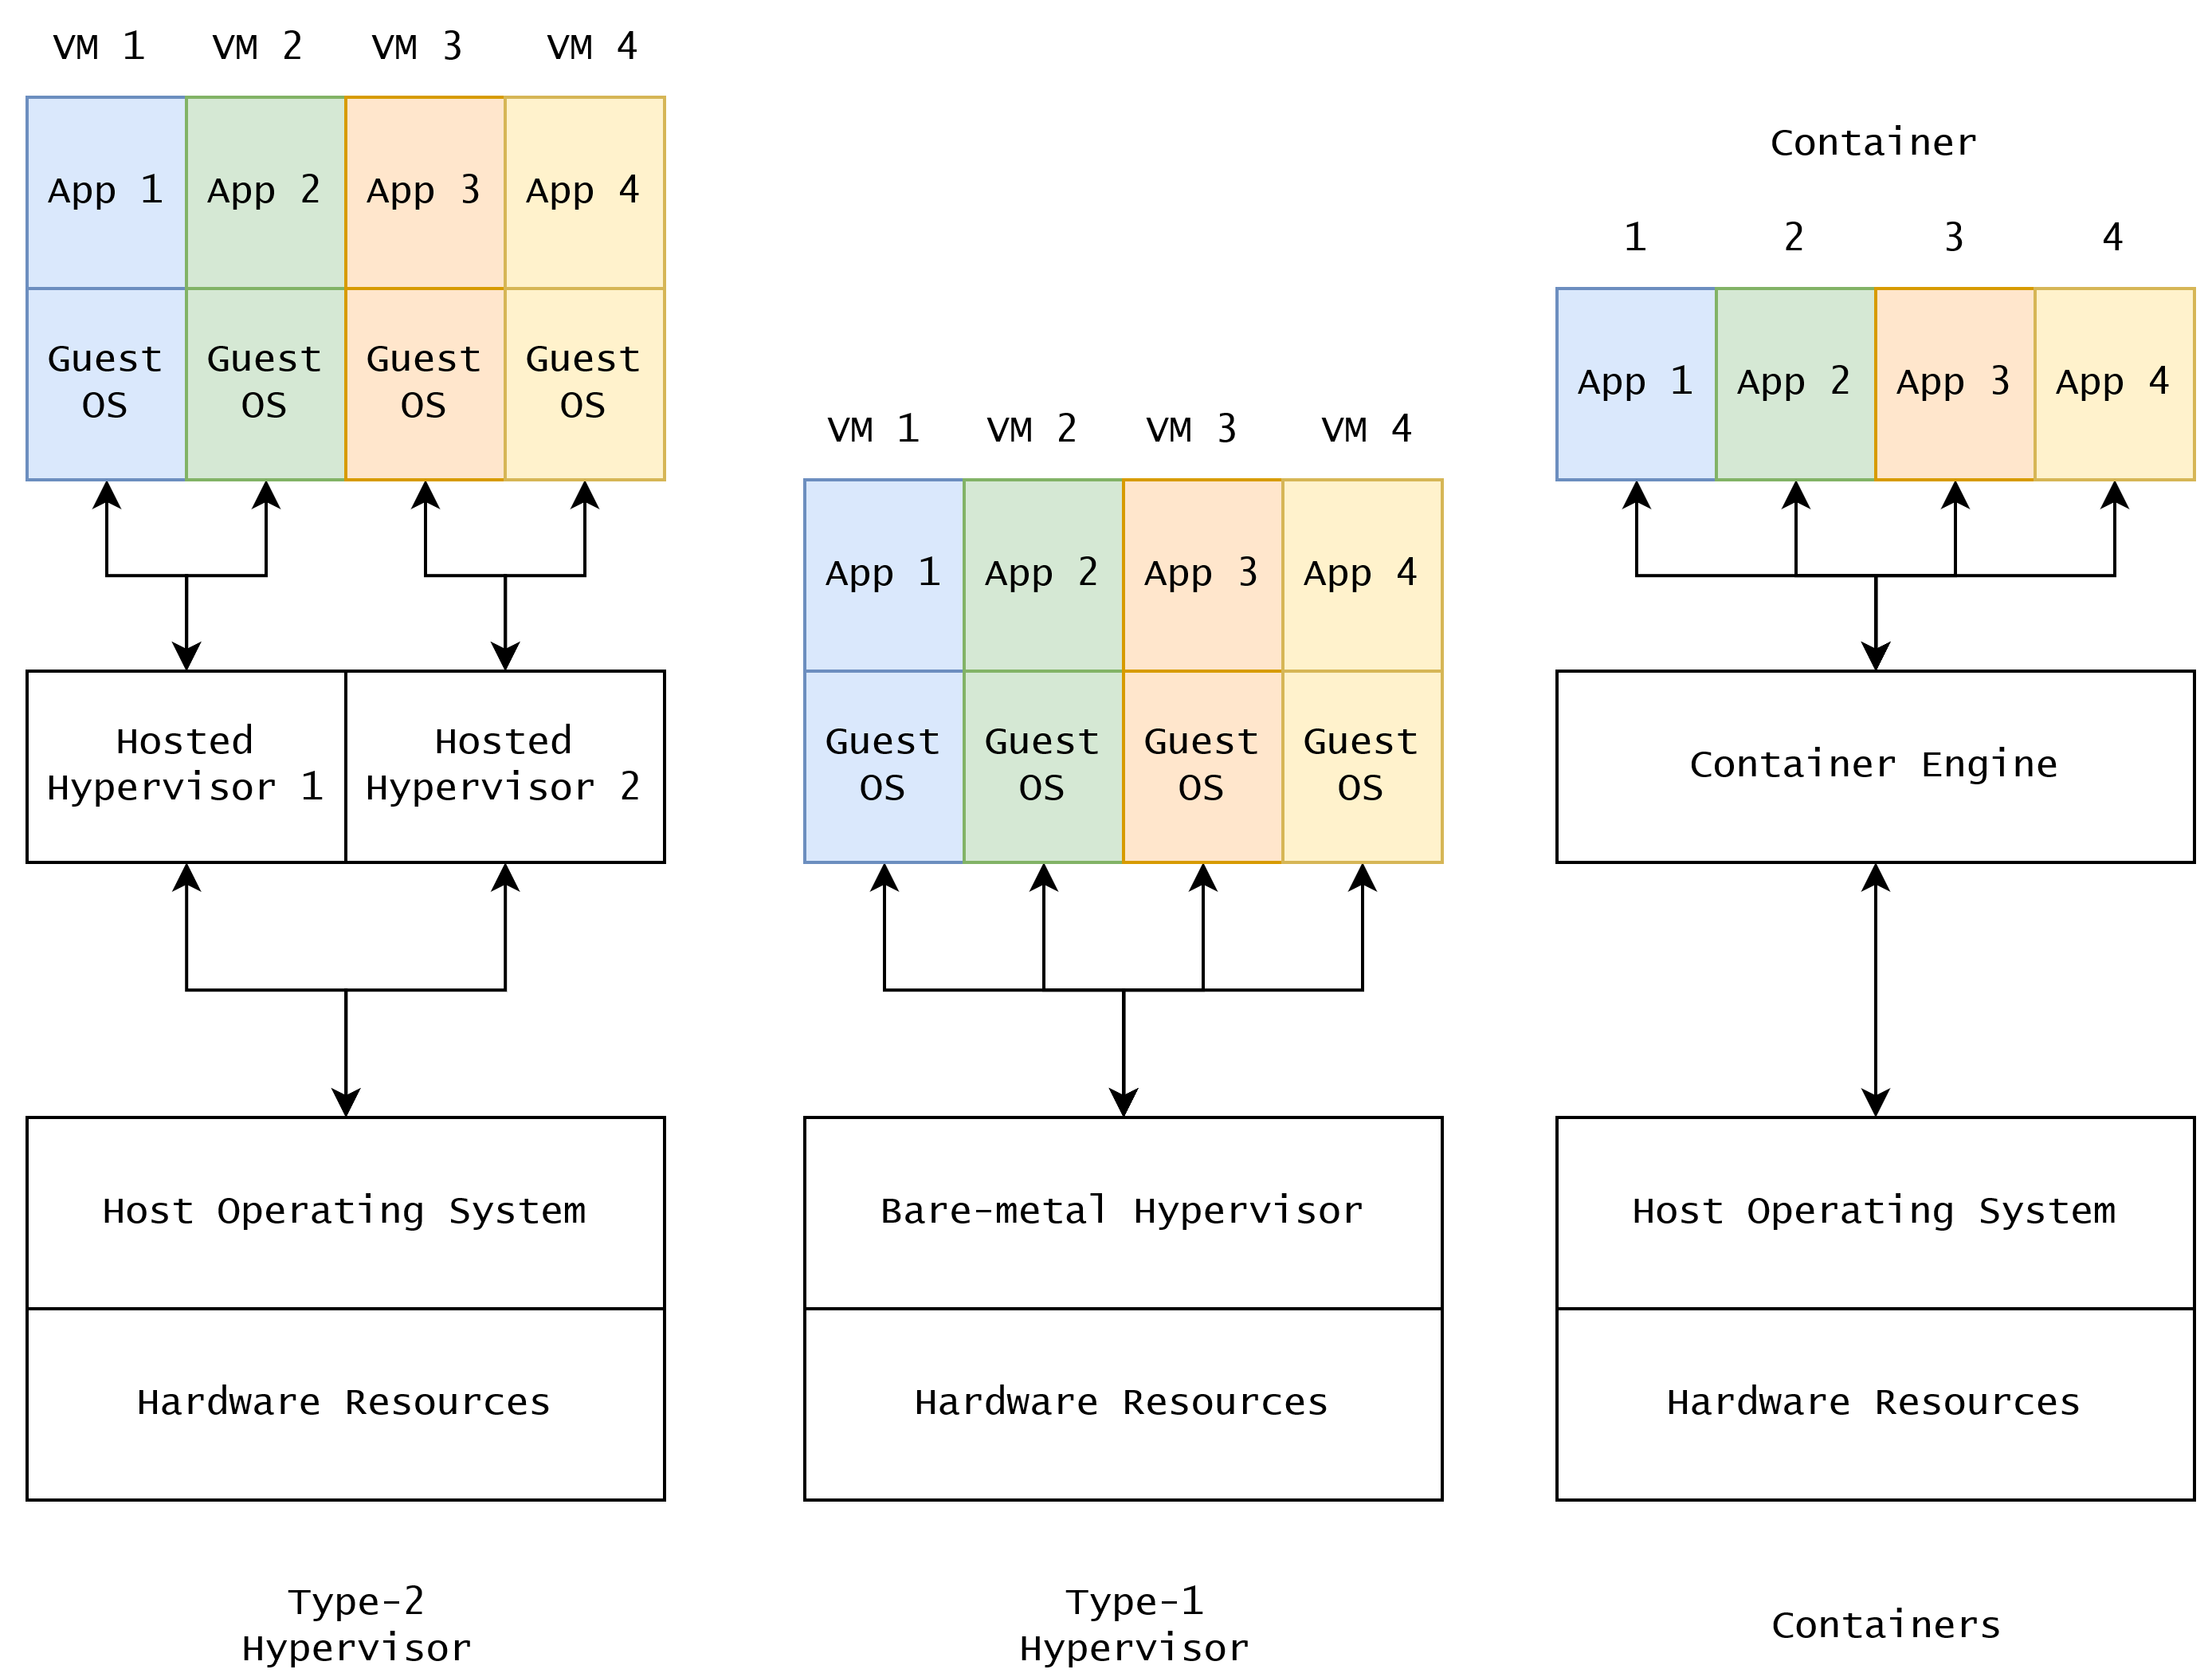
\includegraphics[width=\textwidth]{2_Chapitre2/figures/virtualization.png}
	\caption{Aperçu des différents modèles d'isolation : virtualisation (avec hyperviseurs de types 1 et 2) et conteneurisation.}
	\label{figure:context-virtualization}
\end{figure}

\subsubsection{Machines virtuelles}

La virtualisation assistée par le matériel permet à plusieurs systèmes d'exploitation \textit{invités} complets de fonctionner indépendamment sur des ressources physiques partagées, quelle que soit la nature du système d'exploitation \textit{hôte}~\cite{kivityKvmLinuxVirtual}.

Du point de vue d'une application déployée dans une \gls{VM}, l'environnement d'exécution isolé est perçu comme une plateforme complète, alors qu'il s'agit en réalité d'un sous-ensemble des ressources de la plateforme hôte, déterminé par l'hyperviseur (ou \gls{VMM}, pour \textit{Virtual Machine Manager}), un logiciel de bas niveau qui peut faire office de système d'exploitation, ou s'exécuter en tant que processus du système d'exploitation hôte.

L'hyperviseur a la responsabilité de gérer le cycle de vie des machines virtuelles : la création, l'exécution, la destruction et parfois la migration des machines virtuelles sont gérées par l'hyperviseur.

Les hyperviseurs existent sous deux formes différentes, comme illustré dans la figure~\ref{figure:context-virtualization} :

\begin{itemize}
    \item Les hyperviseurs de type 1 (\textit{bare-metal}) s'exécutent directement sur le matériel de la machine hôte. Étant donné qu'ils ne dépendent pas d'un système d'exploitation (\gls{OS}, pour \textit{Operating System}) sous-jacent, ils sont considérés comme plus sûrs et plus efficaces que leurs homologues hébergés. Parmi les exemples courants d'hyperviseurs de type 1, on trouve VMware ESXi~\footnote{\href{https://www.vmware.com/products/cloud-infrastructure/esxi-and-esx}{https://www.vmware.com/products/cloud-infrastructure/esxi-and-esx}}, Linux KVM~\footnote{\href{http://www.linux-kvm.org/}{http://www.linux-kvm.org/}}, Xen~\footnote{\href{https://xenproject.org/}{https://xenproject.org}} et Microsoft Hyper-V~\footnote{\href{https://learn.microsoft.com/en-us/virtualization/hyper-v-on-windows/about/}{https://learn.microsoft.com/en-us/virtualization/hyper-v-on-windows/about/}} ;
    \item Les hyperviseurs de type 2 (hébergés) s'exécutent au-dessus d'un système d'exploitation. Ces hyperviseurs sont des produits grand public qui offrent aux utilisateurs finaux un moyen pratique d'exécuter des systèmes ou des programmes qui ne seraient pas nativement pris en charge par leur matériel ou leur système d'exploitation. Parmi les hyperviseurs de type 2, on peut citer QEMU~\footnote{\href{https://www.qemu.org/}{https://www.qemu.org}} et Oracle VirtualBox~\footnote{\href{https://www.virtualbox.org/}{https://www.virtualbox.org/}}.
\end{itemize}

\subsubsection{Conteneurs}

La conteneurisation est une technique de virtualisation au niveau du système d'exploitation. Le noyau du système d'exploitation hôte est responsable de l'allocation des ressources. Les conteneurs virtualisent le système d'exploitation : ils donnent au processus conteneurisé l'impression d'avoir toute la machine à leur disposition, tout en étant en réalité contraint et limité en ce qui concerne l'utilisation des ressources par le noyau hôte~\cite{bentalebContainerizationTechnologiesTaxonomies2022}.

Les conteneurs constituent un mécanisme d'isolation léger qui repose sur les capacités d'isolation du noyau du système hôte, comme le montre la figure~\ref{figure:context-virtualization}. En l'occurrence, sous Linux :

\begin{itemize}
    \item \texttt{chroot} : modifie le répertoire racine apparent pour une arborescence de processus donnée. Il permet à un conteneur d'opérer sur un répertoire virtuel \texttt{/} qui pourrait être situé n'importe où sur le système de fichiers de l'hôte ;
    \item \texttt{cgroups} : permettent de créer des groupes hiérarchiques de processus et allouer, limiter et surveiller les ressources matérielles pour ces groupes : E/S vers et depuis les périphériques de bloc, accès à l'unité centrale, à la mémoire et aux interfaces réseau ;
    \item \texttt{namespaces} : une couche d'abstraction autour des ressources du système d'exploitation, telles que le réseau ou les communications entre processus (\gls{IPC}, pour \textit{Inter-Process Communication}). Les processus au sein d'un espace de noms ont leurs propres instances isolées de ces ressources système.
\end{itemize}

L'ambition derrière les conteneurs est de contenir l'exécution d'une application dans un processus isolé du reste du système, de sorte à ce qu'il ignore les autres processus exécutés par le système hôte. Le cycle de vie des conteneurs est géré par un moteur de conteneurs. Le conteneur est amorcé à partir d'une image qui contient toutes les dépendances nécessaires à la construction et/ou à l'exécution de l'application.

Dans l'écosystème des conteneurs, Docker~\footnote{\href{https://www.docker.com/}{https://www.docker.com/}} en particulier a connu une forte progression depuis sa création en 2013. Docker a joué un rôle déterminant dans la spécification des normes industrielles pour les formats de conteneurs par le biais de l'\textit{Open Container Initiative}~\footnote{\href{https://opencontainers.org/}{https://opencontainers.org/}} (OCI), qui définit les spécifications des images de conteneurs - des lignes directrices sur la manière de créer une image OCI avec son manifeste, ses couches de système de fichiers et sa configuration - et les spécifications d'exécution concernant la manière d'exécuter les paquets d'applications au fur et à mesure qu'ils sont décompressés sur le système d'exploitation hôte.

\subsection{Dimensionnement : équilibrage de charge et passage à l'échelle}

Dans le cloud, les applications sont souvent déployées sur plusieurs zones géographiques (différents centres de données), et sur plusieurs nœuds (serveurs) au sein de l'infrastructure~\cite{hayesCloudComputing2008}. Chaque déploiement de l'application est appelé "instance".

Une brique logicielle essentielle dans une plateforme cloud est le \textit{load balancer}. Son rôle est de distribuer les requêtes entrantes (\textit{i.e.} la charge) pour une application entre les différentes instances déployées~\cite{jafarnejadghomiLoadbalancingAlgorithmsCloud2017}. Ce processus doit être transparent du point de vue des utilisateurs de l'application, qui ne savent pas quelle instance répond à leurs requêtes.

L'équilibrage de charge s'appuie sur des politiques (ou stratégies) de gestion des ressources qui peuvent viser différents objectifs. Un fournisseur de services peut chercher à répartir la charge autant que possible de manière à minimiser la latence des requêtes ; à l'inverse, il peut chercher à consolider les tâches sur un nombre réduit de nœuds, afin de réduire la consommation d'énergie de la plateforme~\cite{leeEnergyEfficientUtilization2012}.

Lorsque la charge sur une application augmente, une mise à l'échelle (ou \textit{scaling}) des ressources matérielles qui lui sont allouées peut alors être effectuée selon deux axes :

\begin{itemize}
    \item \textbf{Verticalement}~\cite{boyd-wickizerAnalysisLinuxScalability, linderOracleParallelRDBMS1993, xian-hesunScalabilityParallelAlgorithmmachine1994} : en attachant plus de ressources matérielles aux serveurs qui supportent l'application (par exemple, augmenter le nombre de \gls{CPU} ou la quantité de mémoire alloués à une \gls{VM}). Il peut s'agir de migrer une instance de l'application vers un nouveau serveur plus performant, ce qui a un impact sur la disponibilité de l'application. Le mécanisme d'équilibrage de charge permet de router temporairement les requêtes entrantes vers une instance fonctionnelle de l'application en attendant l'initialisation de la nouvelle instance ;
    \item \textbf{Horizontalement}~\cite{al-faresHederaDynamicFlow, lakshmanCassandraDecentralizedStructured2010, weilCephScalableHighPerformance} : en augmentant le nombre de serveurs alloués à l'application. Le mécanisme d'équilibrage de charge permet d'acheminer les requêtes et les réponses entre les utilisateurs et les multiples instances de l'application.
\end{itemize}

L'opération contraire peut être symétrique, ou non, lorsque le nombre ou la complexité des traitements diminue.

\subsection{Qualité de service et métriques de performances}

Les fournisseurs de services cloud sont souvent tenus à des engagements (\gls{SLA}, pour \textit{Service Level Agreement}) en matière de qualité de service (\gls{QoS}, pour \textit{Quality of Service}). Ils s'engagent auprès de leurs clients sur un certain nombre de critères (\gls{SLO}, pour \textit{Service Level Objective}) mesurés par des métriques telles que la latence, le débit, la disponibilité, etc. En cas de violation de ces engagements, le fournisseur consent généralement une remise au client lésé~\cite{buyyaSLAorientedResourceProvisioning2011}.

Une méthode naïve pour respecter des engagements de qualité de service en matière de performance consiste à ne pas partager les ressources matérielles entre les clients. Ainsi, chaque client reste utilisateur prioritaire sur une machine réservée à son usage. Cette hypothèse est bien entendu incompatible avec l'objectif de profits d'un fournisseur de services, qui mutualise des ressources dans le but précis de réaliser des économies d'échelle (voir section~\ref{section:background-virtualization}).

Ajuster les allocations de ressources est un problème fondamental dans le cloud. Lorsque les clients sont responsables de la réservation des ressources nécessaires à leurs applications, on constate une tendance à réserver plus de ressources que nécessaire, de manière à s'assurer une marge de sécurité~\cite{rzadcaAutopilotWorkloadAutoscaling2020}. Cela pousse les fournisseurs de services à la surréservation~\cite{tomasImprovingCloudInfrastructure2013} (ou \textit{overbooking}), c'est-à-dire à allouer plus de ressources virtuelles à leurs clients que physiquement disponibles dans leur infrastructure. Le corollaire de cette pratique est le phénomène d'\textit{overcommitment}~\cite{bashirTakeItLimit2021} : une dégradation des performances lorsque les ressources réellement utilisées dépassent la capacité réelle des serveurs.

Cet objectif pour un fournisseur de services de minimisation des coûts se heurte à la contrainte de performances, c'est-à-dire la rapidité à laquelle les traitements demandés par les clients sont réalisés. Afin de s'assurer de respecter leurs \gls{SLA}, les fournisseurs de services dimensionnent leurs centres de données en fonction des pics de charge qu'ils anticipent. Ainsi, il n'est pas rare de constater des niveaux d'utilisation des ressources inférieurs à 15\%~\cite{vasanWorthTheirWatts2010, vermaLargescaleClusterManagement2015a}, pour absorber les pannes et les interférences entre charges de travail.

Pour surmonter ce défi, les fournisseurs ont besoin de caractériser précisément les charges de travail~\cite{cortezResourceCentralUnderstanding2017a}. Par exemple, dans le calcul haute performance, on constate l'existence d'un grand nombre de tâches à basse priorité~\cite{tirmaziBorgNextGeneration2020}. Une stratégie d'ordonnancement moins stricte pourrait être adoptée pour une telle classe d'applications.

\section{Vers un nouveau modèle de service pour le cloud}

Dans cette section, nous présentons les limites des plateformes cloud en matière de capacités de mise à l'échelle des ressources allouées aux applications. Nous discutons des architectures logicielles pour les applications déployées dans le cloud, et introduisons un modèle de service émergent qui entend s'appuyer sur un changement architectural pour répondre à la problématique du dimensionnement automatique.

\subsection{La promesse de l'élasticité dans le cloud}

Dans la section précédente, nous avons vu que l'élasticité rapide, au sens de mise à l'échelle dynamique des ressources en adéquation avec les besoins des applications déployées, est considérée par le \gls{NIST} comme une caractéristique essentielle du cloud. Pourtant, elle ne fait pas systématiquement partie des services offerts par les fournisseurs cloud~\cite{herbstElasticityCloudComputing}. Il incombe le plus souvent aux clients de planifier à l'avance et de spécifier leurs besoins, c'est-à-dire de réserver une quantité adéquate de ressources. Ces ressources sont généralement appelées "instances" par les fournisseurs de services cloud. Les instances cloud se distinguent généralement en fonction de leurs spécifications en termes de type de ressources et de capacité : par exemple, on peut trouver des instances avec de nombreux cœurs \gls{CPU}, tandis que d'autres donnent accès à un \gls{GPU} ou autre accélérateur matériel.

La mise à l'échelle automatique des ressources nécessaires à un ensemble d'applications reste un problème ouvert dans la littérature~\cite{straesserWhyItNot2022}. Le choix du ou des types d'instances et de leur quantité pour une application dépend a) de la nature des calculs effectués, et b) de la latence acceptable et du débit souhaité~\cite{yallesRISCLESSReinforcementLearning}. Il est de la responsabilité du client de ne pas surprovisionner ces ressources au-delà de ses besoins réels.

Cette conception de l'offre a plusieurs conséquences. Tout d'abord, cela signifie que la facturation est faite à gros grain : elle est établie par instances réservées, plutôt que par ressources réellement utilisées. En outre, le coût des ressources inactives incombe au client : lorsque l'application ne traite aucune requête, elle reste déployée dans un état dormant, en attente d'une nouvelle demande entrante.

\subsection{Applications dans le cloud : du monolithe aux microservices}

Le cloud a vu naître de nouvelles techniques de développement. Le développement "cloud-native" consiste à construire des applications pour le cloud, en prenant en compte dès leur conception les besoins futurs de mise à l'échelle~\cite{dragoniMicroservicesHowMake2018, martinfowler2014microservices}.

Une application monolithique est construite comme une unité unique, dont les différents services exposés ne sont pas découplés~\cite{villamizarEvaluatingMonolithicMicroservice2015}. Lors de la mise à l'échelle d'un monolithe, l'augmentation du nombre d'instances du monolithe (mise à l'échelle horizontale) peut s'avérer inefficace en termes de coûts, car toutes les parties d'une application ne subissent pas des pics de charge en même temps. Une augmentation des requêtes vers une zone logique de l'application implique une mise à l'échelle de l'infrastructure pour l'ensemble de l'application.

Une architecture logicielle en microservices consiste à organiser une application sous la forme d'une collection de services faiblement couplés~\cite{12factor}. Chacun de ces services s'exécute dans son propre processus, communique avec les autres par le biais du passage de messages et peut être déployé de manière indépendante sur des serveurs hétérogènes afin d'atteindre les objectifs de niveau de service. Une augmentation des requêtes vers une zone logique de l'application peut être absorbée par la mise à l'échelle de l'infrastructure pour ce seul microservice.

L'infrastructure en microservices facilite donc la mise à l'échelle des applications dans le cloud en permettant un déploiement indépendant pour chacune des composantes d'une application~\cite{vaneykSPECRGReferenceArchitecture2019}.

\subsection{Introduction au modèle serverless}

Dans cette section, nous présentons le modèle de service serverless pour le cloud. Nous passons en revue les caractéristiques essentielles des plateformes serverless, et donnons les propriétés qu'une application doit respecter pour un déploiement serverless.

\subsubsection{Caractéristiques des plateformes serverless}

% TOOD: Le modèle serverless n'est pas une idée nouvelle... Première mention de "serverless" dans la littérature~\cite{andersonServerlessNetworkFile}...

Le serverless désigne à la fois un modèle de programmation et un modèle de service pour le cloud. Dans une architecture serverless, les développeurs conçoivent leurs applications comme une composition de fonctions sans état. Sans état (ou "pur", sans effet de bord) signifie que le résultat du calcul dépend exclusivement des entrées~\cite{burckhardtNetheriteEfficientExecution}. Ces fonctions prennent en entrée une valeur et un contexte d'invocation, et produisent un résultat qui est stocké dans un système de stockage. Leur exécution est déclenchée par un événement tel qu'une requête \gls{HTTP}, une tâche planifiée, un téléchargement de fichier, etc. Ainsi, le serverless est un modèle dirigé par les événements~\cite{SchleierSmith2021WhatSC}. Dans les offres commerciales de cloud public, le modèle serverless est souvent appelé \textit{Function as a Service}~\cite{hellersteinServerlessComputingOne2019} (\gls{FaaS}).

L'appellation \textit{serverless} ne signifie pas que des serveurs ne sont plus utilisés pour héberger et exécuter des applications. Le terme fait référence à une abstraction sur les ressources matérielles qui permet aux développeurs de s'affranchir de la gestion des serveurs qui supportent leurs applications. Grâce à des mécanismes de mise à l'échelle automatique, les développeurs sont libérés de la réservation des ressources nécessaires au déploiement de leurs charges de travail~\cite{vaneykSPECRGCloud2018}. Les plateformes serverless sont conçues pour gérer de manière automatique les besoins de mise à l'échelle et ainsi répondre aux fluctuations de la demande sur les applications, évitant ainsi aux développeurs d'avoir à définir des stratégies de mise à l'échelle explicites. L'objectif du modèle est de rapprocher les clients de la logique métier de leurs applications~\cite{vaneykSPECRGReferenceArchitecture2019}.

Une caractéristique nouvelle dans le modèle serverless est celui de mise à l'échelle à zéro : lorsqu'une fonction ne reçoit pas de requêtes entrantes, la plateforme serverless libère les ressources qui lui étaient précédemment allouées. Ainsi, les fournisseurs ne facturent les clients que lorsque leur application utilise effectivement des ressources matérielles~\cite{hellersteinServerlessComputingOne2019}.

Pour permettre la mise à l'échelle à zéro des applications, il est nécessaire que celles-ci soient déployées dans des environnements d'exécution "jetables" : leur durée de vie est inférieure à celle des données sur lesquelles ils opèrent. Les données quant à elles doivent être pérennes, et sont donc sauvegardées sur des stockages persistants. On parle de \textit{désagrégation} de l'état des applications. Ainsi, les plateformes serverless dans le cloud public fournissent un ensemble de logiciels dorsaux (ou \textit{backend}), appelés \gls{BaaS}~\cite{mikeroberts2018serverless} (pour \textit{Backend as a Service}). Ce sont des offres commerciales et gérées par le fournisseur, mises à la disposition des développeurs d'applications pour fournir un ensemble de services à longue durée de vie : bases de données, stockage, bus de messages, etc. Ces services tiers constituent l'infrastructure de base des applications serverless.

L'abstraction offerte par le modèle permet aux fournisseurs de déployer le code de leurs clients dans plusieurs zones géographiques. Ce mécanisme de basculement garantit la disponibilité en cas de panne dans une zone de déploiement et réduit le risque de défaillance d'une fonction dans l'application~\cite{taibiPatternsServerlessFunctions2020}. En outre, comme les instances de fonction sont créées à la demande par le fournisseur, le modèle de concurrence offert par les plateformes serverless signifie que les performances d'une application peuvent évoluer linéairement avec le nombre de requêtes~\cite{mcgrathServerlessComputingDesign2017}.

\subsubsection{Caractéristiques des charges de travail serverless}

Du point de vue du client, le serverless permet une mise à l'échelle automatique de leurs applications. La facturation est effectuée au plus juste, uniquement lorsque les ressources sont effectivement utilisées et pour la durée exacte de l'exécution. Du point de vue du fournisseur, la granularité d'allocation permet un meilleur multiplexage des ressources, ce qui se traduit par une efficacité accrue et donc des bénéfices plus importants.

Mais ce mécanisme de mise à l'échelle automatique a un coût en termes de latence : initialiser de nouvelles instances de fonctions pour les requêtes entrantes peut provoquer des délais, menant à des situations où les temps d'initialisation peuvent dominer les temps d'exécution des fonctions~\cite{Jiang2021TowardsDS}. Par ailleurs, les performances peuvent aussi être dégradées en termes de débit : étant donné que l'état des fonctions doit être sauvegardé dans un stockage désagrégé, les applications qui présentent des motifs de communications entre les fonctions peuvent souffrir du temps de récupération des données dans les nœuds de calcul~\cite{mullerLambadaInteractiveData2020}.

En réponse à ces limites du modèle, la Cloud Native Computing Foundation~\footnote{\href{https://www.cncf.io/}{https://www.cncf.io/}} (\gls{CNCF}), une initiative de la Fondation Linux~\footnote{\href{https://www.linuxfoundation.org/}{https://www.linuxfoundation.org/}} soutenue par plus de 800 membres industriels impliqués dans les services cloud, identifie des propriétés idéales pour les cas d'usage serverless, notamment~\cite{cncf2018whitepaper} :

\begin{itemize}
    \item Charges de travail hautement parallèles, asynchrones et concurrentes, avec peu ou pas de communication et pas de synchronisation entre les processus ;
    \item Tâches de fréquence variable, avec de fortes fluctuations de charge, c'est-à-dire des tâches interactives plutôt que des tâches par lots ;
    \item Processus sans état et éphémères, sans besoin majeur d'un temps de démarrage instantané.
\end{itemize}

Pour ces classes d'applications, un déploiement serverless peut être envisagé comme une alternative efficace en matière de coût par rapport aux modèles traditionnels. Toutefois, elles ne recouvrent pas tous les cas d'usage dans le cloud. Si les possibilités de gestion fine des allocations de ressources semblent donner le serverless comme le futur premier modèle de service dans le cloud~\cite{hellersteinServerlessComputingOne2019}, il apparaît donc que les plateformes serverless soulèvent des défis qui restent à relever.


\section{Conclusion}

Nous avons vu que les offres traditionnelles du cloud reposent sur la réservation de ressources matérielles par les clients. La capacité pour une plateforme à provisionner des ressources à la demande permet aux clients de bénéficier d'une propriété essentielle dans le cloud, l'élasticité. En fonction de la charge (c'est-à-dire le trafic entrant) que subit une application, la plateforme doit permettre d'ajuster la quantité de ressources allouées à l'application, de manière à garantir ses performances.

Cette élasticité n'est généralement pas automatique : il incombe aux clients de faire des prévisions pertinentes dans le cadre de leurs déploiements, et d'ajuster la quantité et la nature des ressources matérielles allouées au plus près de leurs besoins. Cette planification est délicate et une erreur d'estimation peut induire des écarts entre les besoins réels et la capacité allouée. Si les ressources sont surprovisionnées, le client doit supporter un coût financier superflu ; si les estimations sont trop basses, les performances des applications risquent d'en pâtir.

Pour pallier cette limite, un nouveau modèle de service a émergé depuis le milieu des années 2010. Appelé \gls{FaaS}, ou \textit{serverless}, il renverse la responsabilité de l'allocation des ressources dans le cloud. C'est à la plateforme du fournisseur de services d'assigner ces ressources aux applications des clients ou de les libérer, automatiquement, lors de variations de charge. Cela devrait permettre de simplifier la gestion des déploiements pour les clients, tout en autorisant le fournisseur de services à optimiser l'utilisation de ses ressources matérielles.

Si le modèle serverless doit permettre Ce mécanisme n'est pas sans soulever de nouveaux problèmes, notamment en matière de performances. Le chapitre suivant fait état d'un ensemble de défis que les fournisseurs de services doivent relever pour permettre le déploiement d'une variété d'applications sur les plateformes serverless sous contrainte de qualité de service.
